\documentclass{LZU}

%参考文献
\usepackage[backend=biber,gbtverbose=true,
	bibstyle=gbt7714_2005_n,citestyle=gbt7714_2005_n]{biblatex}
\addbibresource{ref.bib}
\renewcommand{\bibfont}{\zihao{5}}

%注意,这里一定要两个大括号,里面的那个大括号用于长标题在封面中的断行
\title{{兰州大学本科论文非官方 \LaTeX 模板}}
\entitle{{The unofficial \LaTeX{} template for }{the undergraduate thesis of}{Lanzhou University}}
\author{沈周}

\advisor{导师}
\college{学生所属学院}
\major{专业}
\grade{年级}

%package
\usepackage{minted} %代码格式
\usepackage{dirtree}
\usepackage{siunitx}
\usepackage{hologo}
\usepackage{manfnt}

%math package
\usepackage[math-style=TeX, bold-style=ISO]{unicode-math}
\setmathfont{xits-math.otf}
\newcommand{\bvec}[1]{\symbf{#1}}

\newenvironment{note}{\par\itshape\noindent{\makebox[-5pt][r]{\scriptsize\color{red!90}\textdbend\quad}}}{\par}

\newcommand{\filename}[1]{{\ttfamily #1}}
\newcommand{\package}[1]{{\sffamily #1}}

\newtheorem{question}{Q}
\newtheorem*{answer}{A}

\begin{document}
\maketitle
\makestatement
\frontmatter
\ZhAbstract{你好,这个论文的\LaTeX 模板啊,是我根据论文的要求自己写的,凑活着用呗。好像还是不够长,再写两句。写什么呢。}{你好;好的}
\EnAbstract{
As the first command of the paragraph. This might come in handy when you start a document with body text and not with a sectioning command.

Be careful, however, if you decide to set the indent to zero, then it means you will need a vertical space between paragraphs in order to make them clear. The space between paragraphs is held in , which could be altered in a similar fashion as above. However, this parameter is used elsewhere too, such as in lists, which means you run the risk of making various parts of your document look very untidy by changing this setting. If you want to use the style of having no indentation with a space between paragraphs, use the parskip package, which does this for you, while making adjustments to the spacing of lists and other structures which use paragraph spacing, so they don't get too far apart. If you want both indent and break, use
}{hello, world}
\tableofcontents
\mainmatter
\chapter{简介Introduction}
这是作者在2015年8月借学习《\citetitle{latextutorial}》\cite{latextutorial}一书之机,也为来年毕业论文之备写的一份{\it 非官方}模板。
\begin{note}
    在使用本模板之前,请仔细阅读本文档。并且请\textbf{不要}试图自己编译此文档(你是不会成功的)。
\end{note}
本文档最新编译时间:\today。

\chapter{模板使用}
\section{你好,世界(hello, world)}
首先,我们给出使用本模板的一个最简单的例子,见代码清单\ref{lst:simplest}。

\begingroup
    \captionof{listing}{此模板的一个最简单的例子}
    \label{lst:simplest}
    \inputminted[breaklines,frame=single,linenos]{latex}{simplest.tex}
\endgroup
此代码清单\ref{lst:simplest}保存在\filename{simplest.tex}中,可以安以下过程编译:
\begin{minted}{bash}
    xelatex simplest.tex
    biber simplest
    xelatex simplest.tex
    xelatex simplest.tex
\end{minted}
在Linux系统中,可以直接输入
\begin{minted}{bash}
    make simplest
\end{minted}
或者在Windows系统中,运行\filename{compile.bat}以自动完成上述过程。
\begin{note}
此模板是在TeXLive 2015环境下编写调试的,所以在更低的版本中可能会出现细节上的不同。
\end{note}

\section{文件结构}
\dirtree{%
    .1 ./.
    .2 template.tex\DTcomment{主文件}.
    .2 LZU.cls\DTcomment{cls模板文件}.
    .2 LZU.cfg\DTcomment{配置文件}.
    .2 pic/.
    .3 lzu.eps\DTcomment{校名图片}.
    .2 Makefile\DTcomment{Linux自动编译脚本}.
    .2 compile.bat\DTcomment{Windows自动编译脚本}.
    .2 gbt7714\_2005.def\DTcomment{参考文献格式配置}.
    .2 gbt7714\_2005\_n.bbx\DTcomment{参考文献格式配置}.
    .2 gbt7714\_2005\_n.cbx\DTcomment{参考文献格式配置}.
}
\section{参考文献}
参考文献的格式是按照GB/T 7714-2005标准的。需要三个额外的格式配置文件:\filename{gbt7714\_2005.def}、\filename{gbt7714\_2005\_n.bbx}和\filename{gbt7714\_2005\_n.cbx}。调用的方法为在导言区加入:
\begin{minted}{latex}
    \usepackage[backend=biber,gbtverbose=true,
    bibstyle=gbt7714_2005_n,citestyle=gbt7714_2005_n]{biblatex}
    \addbibresource{ref.bib}
    \renewcommand{\bibfont}{\zihao{5}}
\end{minted}
其中\filename{ref.bib}是论文的\hologo{BibTeX}文件。

例如《\citetitle{latextutorial}》\cite{latextutorial}在\filename{ref.bib}中为
\begin{minted}{bibtex}
@book{latextutorial,
    author ={刘海洋},
    year={2013},
    month={6},
    title={\LaTeX 入门},
    publisher ={电子工业出版社},
    address={北京},
    usera={M}
}
\end{minted}
\begin{note}
    在使用时,\hologo{BibTeX}文件中要多输入一个文献类型标识的域usera,其值请查看\cref{subsec:reference}。并且请仔细检查生成的引用条目,因为直接从Google Scholar等网站拷贝下来的\hologo{BibTeX}条目可能会缺少某些必要的域(比如对于书籍类型的条目会缺少address域)。
\end{note}
\section{字体}
\subsection{中文字体}
格式要求中用到的中文字体有宋体和黑体,但没有规定是什么宋体,什么黑体\footnote{市面上能见到的宋体和黑体至少有几十种。}所以默认情况不做特殊约定,\package{ctex}将根据系统自行选择。
\begin{note}
    由于需要加入封面,所以系统{\bf 必须}安装微软雅黑字体。
\end{note}

当然本模板也提供了两种字体选项:
\begin{enumerate}
    \item windowsnew\\
        使用中易字体和微软雅黑字体。问题是有些地方用到了加粗的宋体,而中易宋体只有一种字重,所以\package{ctex}会使用伪粗体,排版效果不好。
    \item fandol\\
        使用 Fandol 中文字体,唯一的问题可能是不是中易字体。
\end{enumerate}
\subsection{英文字体}
格式要求是使用Times New Roman字体。但是Times New Roman 字体和宋体(不论是中易宋体还是Fandol 宋体)相比明显偏粗,所以默认情况没有设置英文字体为Times New Roman。可以在调用宏包时加入times选项。
\subsection{数学字体}
格式要求中并没有对数学字体做出规定,所以默认情况是用 Latin Modern Math 字体。如果想使用和Times New Roman 配套的数学字体。由于Times New Roman不能直接用在数学公式中,建议将数学字体调成基于Timew New Roman 设计的XITS math。可以在导言区加入
\begin{minted}{latex}
\usepackage[math-style=TeX, bold-style=ISO]{unicode-math}
\setmathfont{xits-math.otf}
\end{minted}
来调整数学字体。当然,使用这款字体这也会导致字重偏大情况。

\section{其他}
\subsection{引用}
在模板中已经调用了\package{cleveref}宏包。所以建议用\mintinline{latex}{\cref{***}}的方式引用,如
\begin{minted}[breaklines,frame=single,linenos]{latex}
引用\cref{ssub:figure}中的\cref{fig:chaos}
\end{minted}
引用\cref{ssub:figure}中的\cref{fig:chaos}
\subsection{数学}
模板中预定义的定理环境有
\begin{itemize}
    \item 假设:assumption
    \item 定义:definition
    \item 命题:proposition
    \item 引理:lemma
    \item 定理:theorem
    \item 公理:axiom
    \item 推论:corollary
    \item 例:example
    \item 猜想:conjecture
\end{itemize}
\subsubsection{一个例子}
\begin{minted}[breaklines,frame=single,linenos]{latex}
\begin{theorem}[斯托克斯公式]
    \begin{equation}
        \int_M d\omega = \int_{\partial M} \omega
    \end{equation}
    \label{thm:stokes}
\end{theorem}
\begin{proof}
    证明详见\citetitle{stokes}\cite{stokes}。
    \qed
\end{proof}
在三维情况下由\cref{thm:stokes}就可以得到\cref{crl:gauss}
\begin{corollary}[高斯公式]
    \[\iiint_{\Omega}\left(\frac{\partial P}{\partial x}+\frac{\partial Q}{\partial y}+\frac{\partial R}{\partial z}\right)dv=\iint_{\Sigma}P\,dy\wedge dz+Q\,dz\wedge dx+R\,dx\wedge dy\]
    \label{crl:gauss}
\end{corollary}
\end{minted}

\begin{theorem}[斯托克斯公式]
    \begin{equation}
        \int_M d\omega = \int_{\partial M} \omega
    \end{equation}
    \label{thm:stokes}
\end{theorem}
\begin{proof}
    证明详见\citetitle{stokes}\cite{stokes}。
    \qed
\end{proof}
在三维情况下由\cref{thm:stokes}就可以得到\cref{crl:gauss}
\begin{corollary}[高斯公式]
    \[\iiint_{\Omega}\left(\frac{\partial P}{\partial x}+\frac{\partial Q}{\partial y}+\frac{\partial R}{\partial z}\right)dv=\iint_{\Sigma}P\,dy\wedge dz+Q\,dz\wedge dx+R\,dx\wedge dy\]
    \label{crl:gauss}
\end{corollary}



\chapter{格式说明}
\label{chp:format}
毕业论文用 A4 标准纸($\SI{210}{mm}\times \SI{297}{mm}$)打印、印刷或复印,按论文顺序装订成册,论文顺序依次为:封面(包括扉页)、诚信责任书、关于毕业论文(设计)使用授权的申明、中文摘要、英文摘要、目录、论文正文、参考文献、附录、致谢、评语。论文页边距一般要求:上边距 \SI{3}{cm}、下边距\SI{2.54}{cm},左右边距\SI{3.17}{cm},页眉页脚\SI{2.0}{cm}。
\section{封面}
论文封面颜色:本科生毕业论文封面统一为白色。

论文题目用三号字,宋体,加粗,其他信息用小三号字,宋体, 加粗,居中。
\section{正文}
\subsection{标题}
\begin{itemize}
    \item 正文标题:一级标题为三号字,黑体,加粗,居中,单倍行距,段前 24 磅,段后 18 磅;
    \item 二级标题为四号字,黑体,顶左,单倍行 距,段前 24 磅,段后 6 磅;
    \item 三级标题为小四号字,黑体,首行缩进2个汉字符,单倍行距,段前12磅,段后6磅。
    \item 正文:采用小四号字,宋体(英文用 Times New Roman 体,12磅),两端对齐,段落首行左缩进2个汉字符,行距20磅,段前段后0磅。
\end{itemize}

\subsection{图表}
\subsubsection{图}
\label{ssub:figure}
图名置于图的下方,五号字,宋体,居中,单倍行距,段前 6 磅,段后 12 磅,图序与图名之间空1个汉字符(如\cref{fig:chaos}所示)。
\begin{figure}
    \centering
    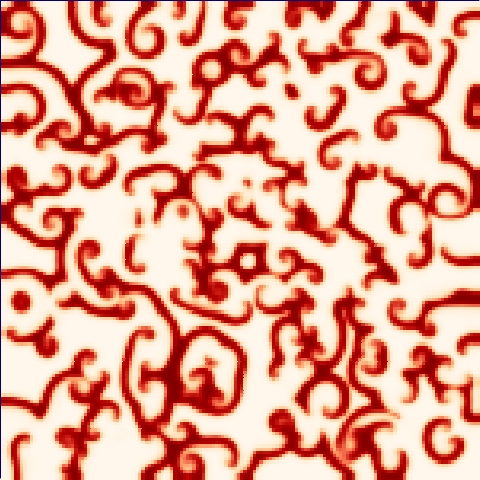
\includegraphics[width=0.5\textwidth]{pic/chaos.png}
    \caption{混沌}
    \label{fig:chaos}
\end{figure}

\subsubsection{表}
表名置于表的上方,五号字,宋体,居中,单倍行距,段 前 6 磅,段后 6 磅,表序与表名之间空 1 个汉字符。表下方的注释 为五号字,宋体,居左(英文用 Times New Roman 体 10.5 磅),单倍行距。
\subsubsection{注释}
一般分为页末注(脚注)和篇末注。脚注,宋体, 9 磅(英 文用 Times New Roman,9 磅),左对齐,单倍行距,段前段后 0 磅, 按阿拉伯数字编号,每页须重新编号。
\subsection{参考文献}
\label{subsec:reference}
参考文献是文中引用的有具体文字来源的文献集合, 毕业论文中引用他人成果之处均应如实、详细地列出参考文献目录。各种主要参考文献按如下格式编排:
\begin{itemize}
    \item 专著、论文集、学位论文、报告:[序号]主要责任者.文献题 名[文献类型标识M/C/D/R].出版地:出版者,出版年.起止页码(任选).
    \item 学术期刊:[序号]主要责任者.文献题名[J].刊名,年,卷 (期):起止页码.
    \item 报纸文章:[序号]主要责任者.文献题名 [N].报纸名,出版日期(版次).
    \item 专利:[序号]专利所有者.专利题名[P].专利国别:专利号,授权日期.
    \item 技术标准:[序号]标准编号,标准名称[S].
    \item 电子文献:[序号]主要责任者.电子文献题名[电子文献和载体类型标识].电子文献的出处或可获得地址,发表或更新日期/引用日期(任选).
\end{itemize}
\section{字体大小测试}
\begin{itemize}
    \item {\zihao{-4}小四}正文
    \item {\zihao{5}五号}正文
\end{itemize}

\backmatter
\printbibliography[title={参考文献},heading=bibintoc]
\Appendix
\section{Q\&A}
\begin{question}
    引用\package{enumerate}宏包之后无法编译通过。
\end{question}
\begin{answer}
    本模板用了\package{enumitem}来重新定义了enumerate环境item之间的距离,使之更符合中文习惯。需要\package{enumerate}宏包来实现的功能\package{enumitem}基本都能实现。如
\begin{minted}{latex}
\begin{enumerate}[label={\roman*.}]
    \item 把编号变成罗马数字。
    \item \package{enumitem}的具体使用请参见该宏包的帮助文档。
\end{enumerate}
\end{minted}
    \begin{enumerate}[label={\roman*.}]
        \item 把编号变成罗马数字。
        \item \package{enumitem}的具体使用请参见该宏包的帮助文档。
    \end{enumerate}
\end{answer}
\section{数学测试}
此处会进行一些输出测试。\footnote{脚注测试}
\begin{itemize}
    \item $\hbar$
    \item $\bvec{a}$
    \item $\int$
    \item \[\fint\intbar\]
\end{itemize}
\Thanks
感谢戴维同学的测试。
\Grade
\end{document}
